
In this section, we compare performance of DPCRT against mbCRT with a case study on peak power reduction.
To this aim, we use the DoE Commercial Reference Building (Doe CRB) simulated in EnergyPlus \cite{DeruFieldStuderEtAl2011} as the virtual test-bed building. 
We first describe our test-bed and introduce the data we use, then validate the quality of the DPCRT modeling on the power consumption prediction of DoE CRB, and finally compare DPCRT and mbCRT on the peak power reduction problem.

\subsection{Test-bed description}
DoE CRB is a large $12$ story office building consisting of $19$ zones with a total area of $500,000$ sq.ft. 
There are $2397$ people in the building during peak occupancy. 
During peak load conditions the building can consume up to $1.6$ MW of power. 
For the simulation of the DoE CRB building we use actual meteorological year data from Chicago for the years $2012$ and $2013$. 
The dataset we use for training the trees can be divided into four different categories:
\begin{enumerate}[leftmargin=1cm]
	\item \textbf{Weather Data:} $w = [\mathrm{w}_1,\ldots,\mathrm{w}_d]$. These data include measurements of the outside dry-bulb and wet-bulb air temperature, relative humidity, and wind characteristics. Since we are interested in predicting the power consumption for a finite horizon, we include the weather forecast of the complete horizon in the training features.
	\item \textbf{Schedule Data:} $s = [\mathrm{s}_1,\ldots,\mathrm{s}_r]$. We create proxy variables which correlate with repeated patterns of electricity consumption, e.g. due to occupancy or equipment schedules. For example, Day of Week is a categorical predictor which takes values from $1$ to $7$ depending on the day of the week. This variable can capture any power consumption patterns which occur on specific days of the week. Likewise, Time of Day is quite an important predictor of power consumption as it can adequately capture daily patterns of occupancy, lighting and appliance use without directly measuring any one of them. Besides using proxy schedule predictors, actual building equipment schedules can also be used as training data for building the trees.
	\item \textbf{Building Data:} $b = [\mathrm{b}_1,\ldots,\mathrm{b}_m]$. These data include the states of the building, such as Chilled Water Supply Temperature, Hot Water Supply Temperature, Zone Air Temperature, Supply Air Temperature and Lighting levels.
	\item \textbf{Power Consumption:} $P$. This is the response variable, in addition to zone temperatures. 
\end{enumerate}
In order to predict the power consumption of the building for the entire length of the horizon, we use the notion of auto-regressive trees. An auto-regressive tree is a regular regression tree except that the lagged values of the response variable are also predictor variables for the regression tree, i.e. the tree structure is learned to provide the following model as in \eqref{eq:RTmodel}
\begin{equation}\label{eq:building_model}
P_t = f \left( w(t), s(t), b(t), P(t-1),\dots, P(t-\delta) \right),
\end{equation}
where $\delta$ is the order of the auto-regression and $P(t-j)$ is the value of the power measured at time $t-j$. 
This allows us to make finite horizon predictions of power consumption for the building.

\subsection{DPCRT modeling validation}

Applying \eqref{E:DPC_split_rule2}, we build multi-variate regression trees using a training dataset from July $2012$. 
For a tree with order of auto-regression $\delta = 6$, a prediction horizon $N = 20$ and $\mathrm{Q}$ equal to the identity matrix, the results on the test dataset are shown in Fig. \ref{F:perf_test}. 
The test set shows a day from July 2013. 
In particular, we compare the building power consumption $P_t$ predicted at time $t$, with the actual power consumption of the building from the test dataset. 
Since we can predict the power for multiple steps of the horizon, we add to the comparison the power prediction at time $t$ computed at $t-10$ and $t-20$, i.e. $P_{t|t-10}$ and $P_{t|t-20}$ respectively. 
It can be seen that even with a relatively long horizon, the multi-variate tree model captures the rapid changes in the response variable very accurately. 
DPCRT uses only a subset of features to train the tree, while the inputs are used to train models in the leaves. Thus, the performance of DPCRT depend on two key assumptions
\begin{itemize}[leftmargin=0.5cm]
	\item the separation of variables does not introduce significant errors while training the tree, and
	\item the linear regression at the leaves is a valid assumption.
\end{itemize}
We verify the validity of these assumptions in terms of their effect on model accuracy considering the following two cases:

\begin{figure}
	\subfigure[Building power consumption at time $t$ predicted at time $t$ is denoted by $P(t)$, predicted 10 steps ahead at time $t-10$ is denoted by $P_{t|t-10}$, and predicted 20 steps ahead at time $t-20$ is denoted by $P_{t|t-20}$.]{
		\centering
		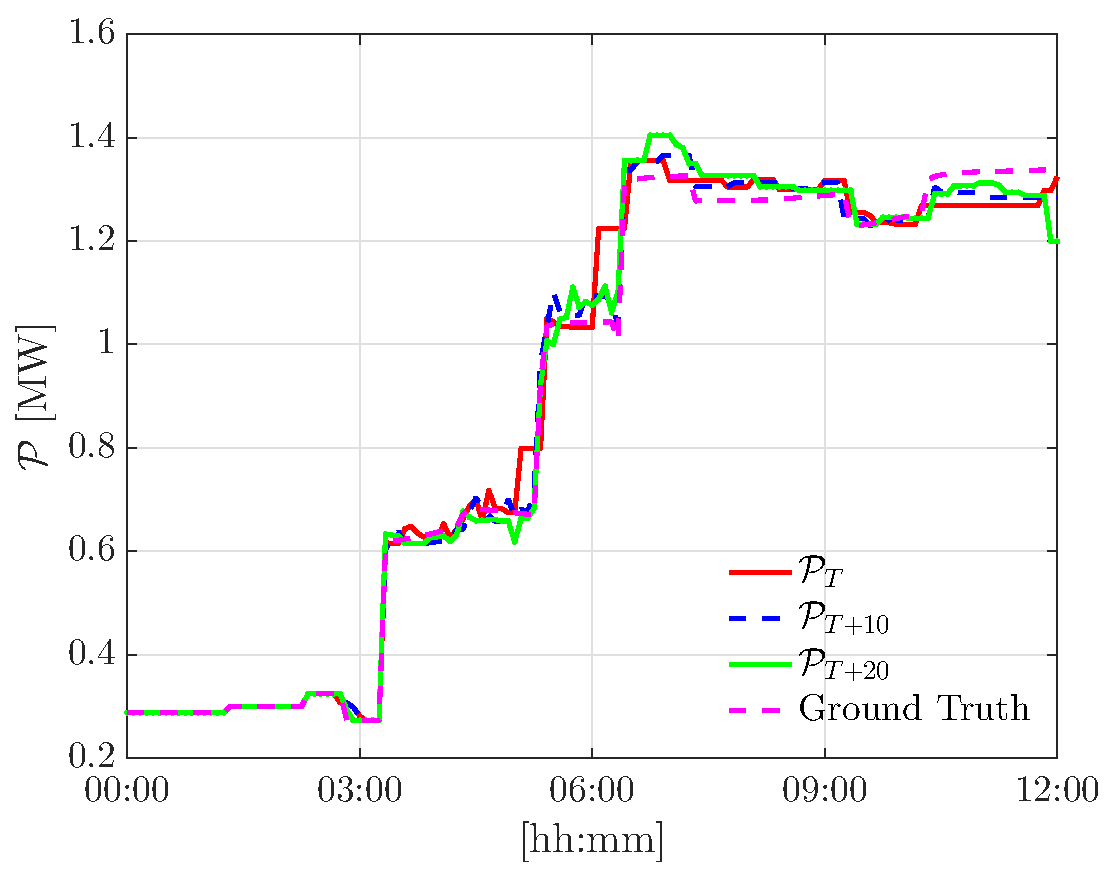
\includegraphics[width=15.7pc]{Figures/perf_test.eps}
		\label{F:perf_test}
	}\hspace{5pt}
	\subfigure[A comparison of power consumption of the building for two different regression trees. $\mathcal{T}_1$ is trained on all the features while $\mathcal{T}_2$ is trained only on non-manipulated features using separation of variables.]{
		\centering
		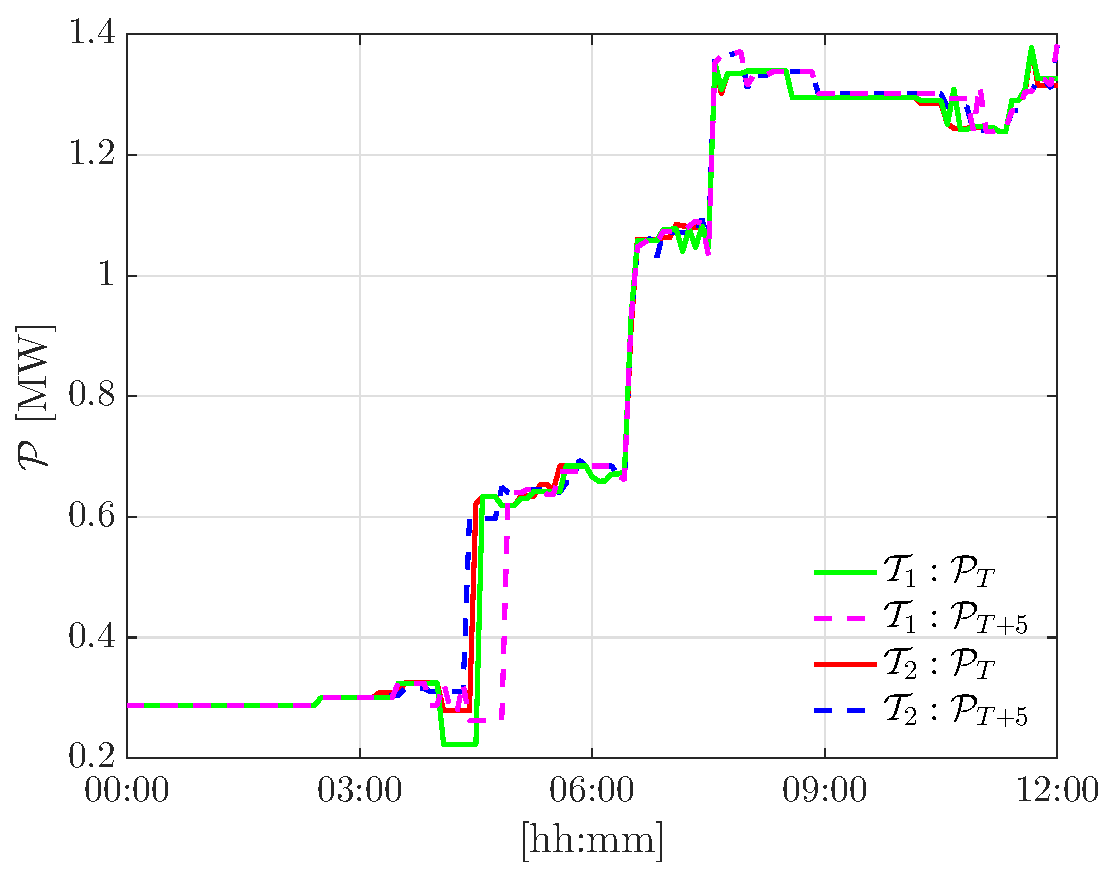
\includegraphics[width=15.7pc]{Figures/separation_vars.eps}
		\label{F:separation_vars}
	}\hspace{5pt}
	\subfigure[Model validation for linear regression at the leaves of the tree. The predicted and the actual power consumption are very close.]{
		\label{F:linear_approx2}
		\centering
		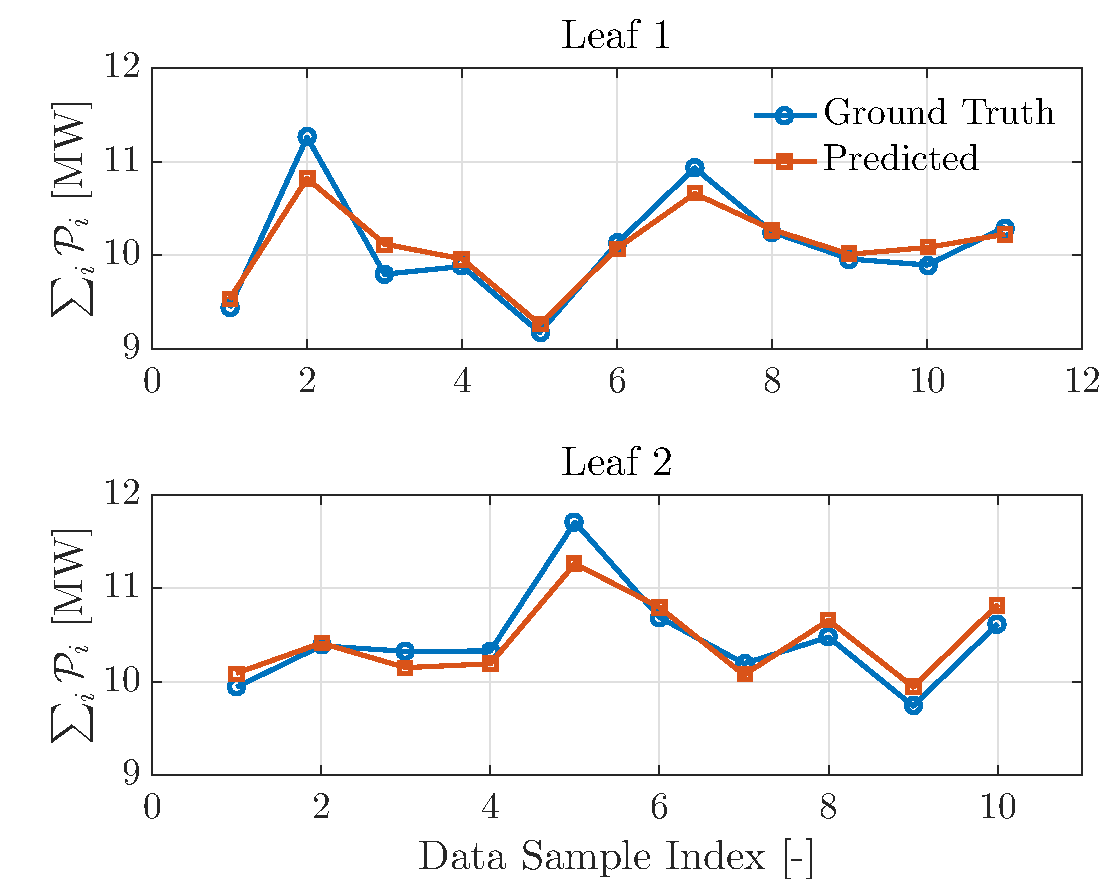
\includegraphics[width=15.7pc]{Figures/error_leaf2_1.eps}
	}\hspace{5pt}
	\subfigure[The tree has 703 leaves. For each leaf, a maximum and a minimum difference in prediction of average power consumption over the control horizon $P_{\mathrm{pred}}-P_{\mathrm{real}}$ is calculated from the data points that end up in that leaf.]{
		\centering
		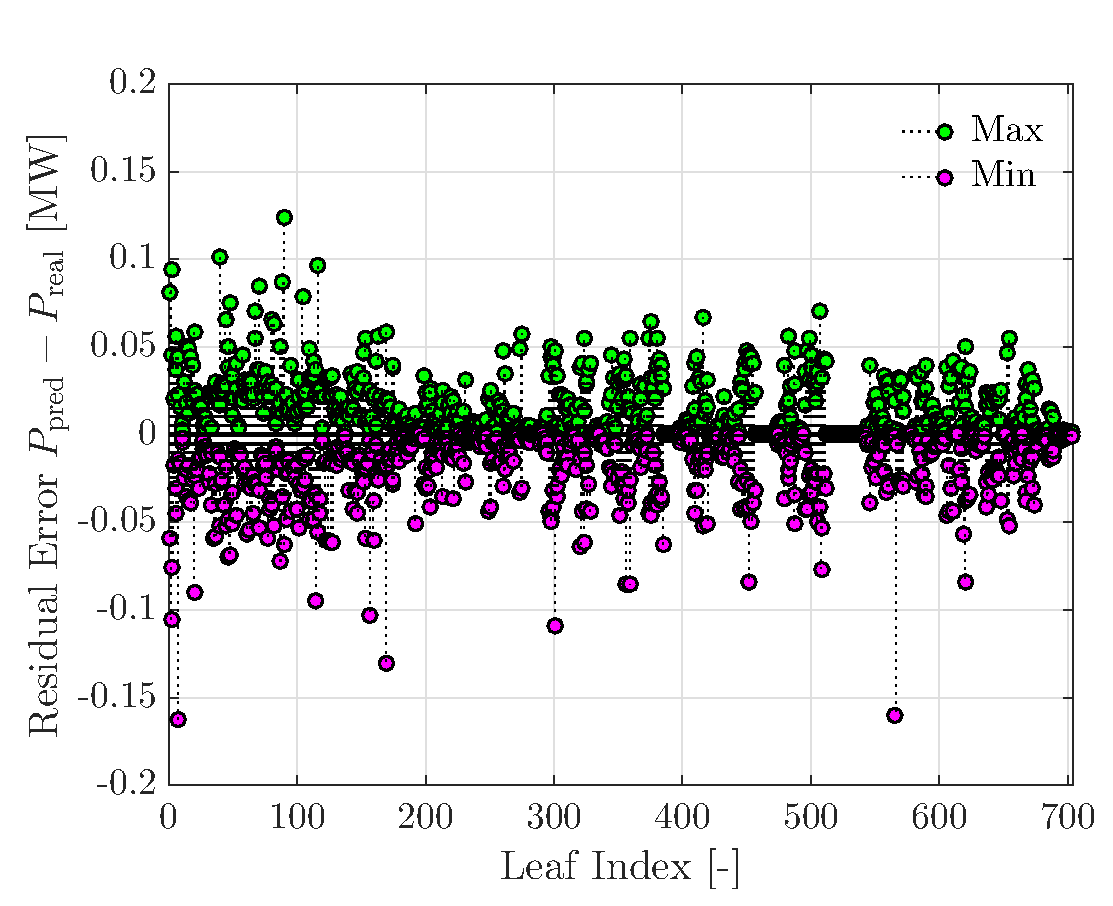
\includegraphics[width=15.7pc]{Figures/error_leaf.eps}
		\captionsetup{justification=centering}
		\label{F:linear_approx}
	}\hspace{5pt}
	\caption{Model Validation of DPCRT.}
	\captionsetup{justification=centering}
\end{figure}

\begin{enumerate}[leftmargin=1cm]
\item We train $2$ kinds of regression trees: $\mathcal{T}_1$, that is trained using all the features described above, and $\mathcal{T}_2$, that was learned from disturbance variables only, with a linear model on the control variables at the leaves as in \eqref{eq:train_model_multi}.
The predicted power consumption of the building at time $t$ and $t+5$, i.e. $P_t$ and $P_{t+5}$, for both trees is shown in Fig. \ref{F:separation_vars}. 
The normalized root mean square error (NRMSE) for these $2$ outputs on the test dataset is shown in Tab. \ref{T:NMRSE_separation_vars}. 
We notice a small loss in model accuracy with $\mathcal{T}_2$ due to the separation of variables.
This is the cost we have to pay for integrating control synthesis with the tree, since otherwise the control features would have been a part of the splitting criteria rather than a linear model in the leaves of the tree.
\item For the tree $\mathcal{T}_2$, we fit a linear model on the sum of all outputs, i.e. the sum of power consumption over the complete control horizon. For each leaf $i$ we have
\begin{gather}
P_t+ \dots + P_{t+N}  = \beta_{0,i} + \beta_i^\top u.
\end{gather}
For $2$ randomly selected leaves, the fit of the linear model against the actual power consumption is shown in Fig.~\ref{F:linear_approx2}. 
The error observed in the predicted and actual power consumption for all leaves is shown in Fig.~\ref{F:linear_approx}. 
It can be seen that for a small number of samples in the leaves of the tree the linear model assumption is valid.
\end{enumerate}

\begin{table}
	\centering
	\caption{NRMSE for regression trees with and without control features.}
	\begin{tabular}{c|c|c|c|c|c|c}
		\toprule
		& $P_t$ &$P_{t+1}$ &$P_{t+2}$ &$P_{t+3}$ &$P_{t+4}$ & $P_{t+5}$ \\
		\midrule
		$\mathcal{T}_1$     & 0.1037  &  0.1036 &   0.1116 &   0.1124 &   0.1140  &  0.1164  \\
		$\mathcal{T}_2$     & 0.1156  &  0.1182 &   0.1270 &   0.1268 &   0.1324  &  0.1308  \\
		\bottomrule
	\end{tabular}
	\label{T:NMRSE_separation_vars}
\end{table}

\subsection{DPCRT for peak power reduction}

The key to answering the question of what actions to take to achieve a significant DR curtailment upon receiving a notification lies in making accurate predictions about the power consumption response of the building. 
In this context, we evaluate the performance of DPCRT for peak power reduction in buildings, and we show the advantages of receding horizon control with regression trees (DPCRT) with respect to the one-step lookahead control (mbCRT). 

As already described, the data samples consist of four types of features, namely weather data, schedule data, building data and autoregressive terms of building power consumption. 
We use the following three features from the building bata as control variables: zone temperature cooling set point $\mathrm{u}_c$ [$^{\circ}$C], chilled water temperature set point $\mathrm{u}_h$ [$^{\circ}$C], and lighting set point $\mathrm{u}_\ell$ (ranges from $0$ to $1$). Since the power consumption model also depends on the zone temperatures, to have a prediction of the power over the horizon, we first need to predict zone temperatures. To this aim, we built two kind of trees with output as power and zone temperature (one for each zone). In the leaf of each tree, we further have three kinds of models as described below.
\begin{itemize}[leftmargin=0.5cm]
	\item The power tree is learned using all the features except for the inputs. In the leaf of the tree, following linear models are trained:
\begin{itemize}[leftmargin=0.5cm]
	\item $P_j^c$ - power consumption at time $j$ due to $\mathrm{u}_c$. 
	Only $\mathrm{u}_c$ have been used to fit the linear model in the leaves.
	\item $P_j^h$ - power consumption at time $j$ due to $\mathrm{u}_h$. 
	Only $\mathrm{u}_h$ have been used to fit the linear model in the leaves.
	\item $P_j^\ell$ - power consumption at time $j$ due to $\mathrm{u}_\ell$.
	Only $\mathrm{u}_\ell$ have been used to fit the linear model in the leaves.
\end{itemize}
\item The temperature tree for the $i^{th}$ zone is learned using all the features except for the inputs and except for the room temperatures $r,\ \forall r\neq i$.
\begin{itemize}[leftmargin=0.5cm]
	\item $T_{i,j}^c$ - temperature of the $i^{th}$ zone at time $j$ due to $\mathrm{u}_c$. 
	Only $\mathrm{u}_c$ have been used to fit the linear model in the leaves.
	\item $T_{i,j}^h$ - temperature of the $i^{th}$ zone at time $j$ due to $\mathrm{u}_h$. 
	Only $\mathrm{u}_h$ have been used to fit the linear model in the leaves.
	\item $T_{i,j}^\ell$ - temperature of the $i^{th}$ zone at time $j$ due to $\mathrm{u}_\ell$. 
	Only $\mathrm{u}_\ell$ have been used to fit the linear model in the leaves.
\end{itemize}
\end{itemize}
With \(u\) defined as $u=[\u_c,\u_h,\u_\ell]^\top$, we can setup the following DPCRT problem to minimize the peak power consumption
\begin{align}
\begin{aligned}
&\underset{u_{t+k}}{\text{minimize }} && \sum_{k=0}^N \frac{P_{t+k}^c + P_{t+k}^h + P_{t+k}^\ell}{3} +
										  \sum_{k=0}^N \sum_{i=1}^{19} \lambda_i \left(\frac{T_{i,t+k}^c+T_{i,t+k}^h+T_{i,t+k}^{\ell}}{3} - T_{ref} \right)^2      \\ 
&\text{subject to }                   && T_{i,t+k}^c                = \alpha_{0,i}^c + \alpha_{i}^c [\u_{c,t},\ldots,\u_{c,t+k}]^\top, i = 1,\ldots,19             \\
&                                     && T_{i,t+k}^h                = \alpha_{0,i}^h + \alpha_{i}^h [\u_{h,t},\ldots,\u_{h,t+k}]^\top, i = 1,\ldots,19             \\
&                                     && T_{i,t+k}^\ell             = \alpha_{0,i}^\ell + \alpha_{i}^\ell [\u_{\ell,t},\ldots,\u_{\ell,t+k}]^\top, i = 1,\ldots,19 \\
& 									  && \sum_{k=0}^N P_{t+k}^c     = \gamma_0^c + \gamma_1^c [\u_{c,t},\ldots,\u_{c,t+k}]^\top 								   \\
& 									  && \sum_{k=0}^N P_{t+k}^h     = \gamma_0^h + \gamma_1^h [\u_{h,t},\ldots,\u_{h,t+k}]^\top 								   \\
&									  && \sum_{k=0}^N P_{t+k}^\ell  = \gamma_0^\ell + \gamma_1^\ell [\u_{\ell,t},\ldots,\u_{\ell,t+k}]^\top 					   \\
&									  && u_{t+k}                   \in [u_{\mathrm{min}},u_{\mathrm{max}}] 																		   \\ 
&									  &&  k                         =  0, \ldots, N.                                                                                \\
\end{aligned}
\label{eq:DPCRTCaseStudy}
\end{align}
At time $t$, we solve DPCRT \eqref{eq:DPCRTCaseStudy} and apply only the first input, i.e. $\u_c(t) = \u^*_{c,t}$, $\u_h(t) = \u^*_{h,t}$ and $\u_\ell(t) = \u^*_{\ell,t}$. At $t+1$, we repeat the algorithm with the updated measurements.

We compare DPCRT and mbCRT when simulated in closed-loop with the EnergyPlus model of the building. In order to compare the performance of DPCRT, we consider a scenario in which there is a significant disturbance which is only anticipated $30$ min in advance and leads to a sudden increase in zone temperatures in the building. This maybe due to a sudden spike in the occupancy or equipment being switched ON at a brief notice. Under this scenario, it is important to react to the disturbance in a predictive manner in order to minimize the peak power consumption. This scenario is shown in Fig. \ref{F:scenario}. Between $15{:}30$ and $16{:}00$, an enormous spike in the power consumption ($1.5\times$) is expected because of a scheduled operation.
\begin{figure*}
	\centering
	\hspace{1pt}
	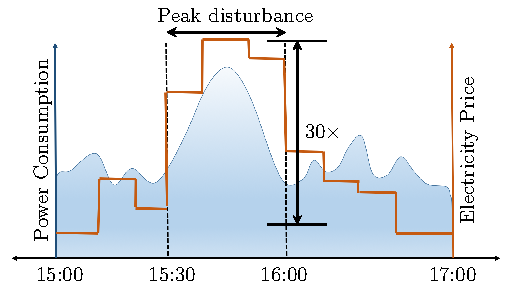
\includegraphics[width=0.5\textwidth]{figs/peakpowerplot.pdf}
	\centering
	\caption{Peak disturbance between $1530-1600$ hours. The test scenario used in the DPCRT case study simulations has a $1.5\times$ peak disturbance between $15{:}30$ and $16{:}00$.}
	\label{F:scenario}
	\vspace{-10pt}
\end{figure*}
\begin{figure}[b!]
\centering
\subfigure[Control strategies.]{
\centering
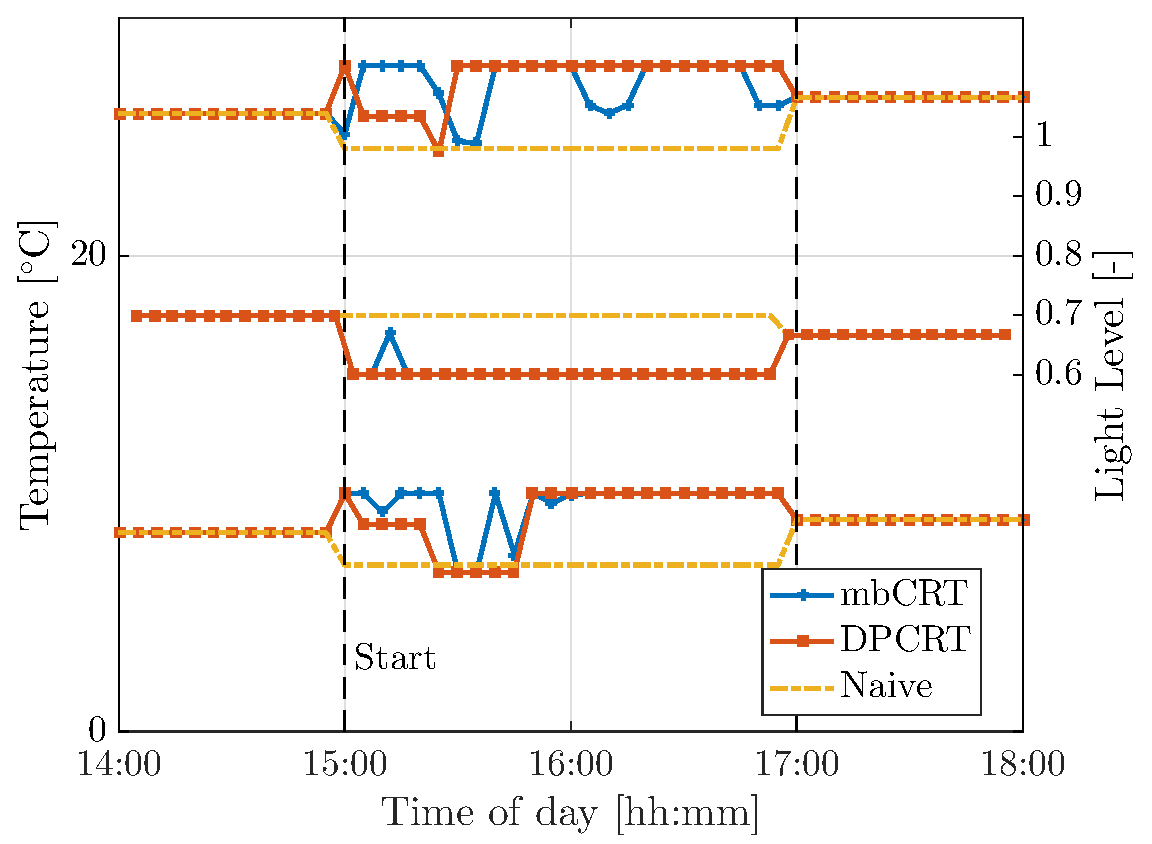
\includegraphics[width=18.5pc]{Figures/res_control.eps}
\label{F:res_control}
}
\subfigure[Power consumption.]{
\centering
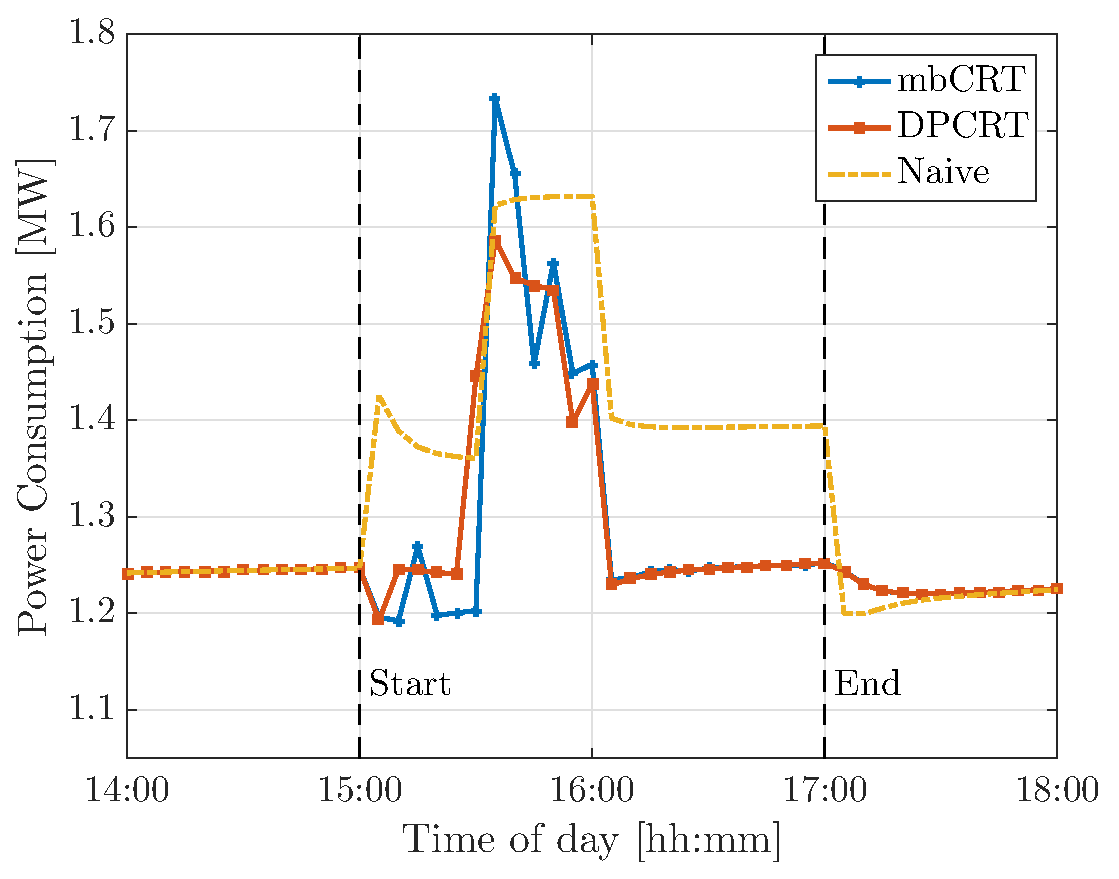
\includegraphics[width=18.5pc]{Figures/res_power.eps}
\label{F:res_power}
}
\caption{A comparison between mbCRT and DPCRT along with a Naive rule-based strategy.}
\captionsetup{justification=centering}
\end{figure}
The control strategies are tested over a $2$ hours duration between $15{:}00$ and $17{:}00$. Fig. \ref{F:res_control} shows $3$ control strategies: mbCRT, DPCRT and a Naive load reduction strategy. The naive strategy is equivalent to not responding to the disturbance at all. It maintains the desired zone temperature set point $\u_c$, chiller water temperature set point $\u_h$ and lighting level $\u_\ell$ throughout the test period. In Fig. \ref{F:res_power}, it can be seen that DPCRT reacts to the disturbance much before mbCRT, which waits until the last time-step before the disturbance to react. This leads to a significantly lower peak power consumption that mbCRT. In the case of DPCRT, the control horizon is $6$. At $15{:}00$, DPCRT strategy is same as the greedy one. At $15{:}05$, the downstream disturbance is visible to DPCRT algorithm and it starts to pre-cool the building by decreasing both cooling and chiller water set points. At $15{:}25$, the $\u_c$ and the $\u_h$ are reduced to minimum so that in the period of extreme disturbance an optimal trade-off between power consumption and thermal comfort is maintained. Thus, DPCRT algorithm foresees the disturbance and takes a preemptive action against it.  On the other hand, the mbCRT algorithm considers the power consumption and the zone temperatures of only one time step. Therefore, it does not know of an upcoming disturbance. At every time step, it chooses that $\u_c$, $\u_h$ and $\u_\ell$ which optimizes the cost for that time step. Naturally, this leads to a jaggy behavior in the control strategy. We can see a similar behavior for the power consumption in Fig. \ref{F:res_power}. The DPCRT algorithm gradually increases the power consumption because it can see the disturbance before it actually reaches $15{:}30$, while in the case of mbCRT, the power consumption overshoots by a big margin because the controller deals with the disturbance in a single step. DPCRT maintains zone temperature much closer to the reference temperature of $24^oC$ while both mbCRT and the naive strategy have large deviations from the desired temperature. 

The quantitative comparison is presented in Tab. \ref{T:case_quant}. Between $15{:}00$ and $17{:}00$, DPCRT and mbCRT result in similar energy usage, $5102$ kWh and $5097$ kWh, respectively, both outperforming the Naive strategy which incurs $5358$ kWh. Peak power in the case of DPCRT is $1.58$ MW which is lower than both mbCRT ($1.73$ MW) and the Naive strategy ($1.63$ MW), although Naive outperforms mbCRT. The peak power with DPCRT is $8.6\%$ less than mbCRT and $3.1\%$ less than the Naive. While both DPCRT and mbCRT account for thermal comfort, DPCRT deviates less from the desired temperature. The Naive strategy does not trade-off on the thermal comfort. Thus, DPCRT outperforms mbCRT both in terms of a reduced peak power consumption and better thermal comfort.

\begin{table}
  \centering
  \caption{Quantitative comparison for Energy Consumption, Peak Power and $\%$ Reduction in Peak Power of DPCRT compared to Naive approach and mbCRT.}
    \begin{tabular}{c|c|c|c}
    \toprule
     & Energy & Peak Power & Peak                       \\
     & [kWh]  & [MW]       & Reduction                  \\     
    \midrule
    Naive     & $5358$     &  $1.63$ &   $3.1\%$        \\
    mbCRT     & $5097$     &  $1.73$ &   $\bold{8.6\%}$ \\
    DPCRT     & $5102$     &  $1.58$ &   -              \\
    \bottomrule
    \end{tabular}
  \label{T:case_quant}
\end{table}
